\section{Auswertung}

\subsection*{Vorbemerkungen}

Bevor wir mit der Aufzeichnung der eigentlichen Spektren begonnen haben, haben wir eine Dunkelstrommessung durchgeführt. Das Spektrum dieser ist in \abbref{fig:dunkelstrommessung} zu sehen.

\begin{figure}[H]
  \centering
  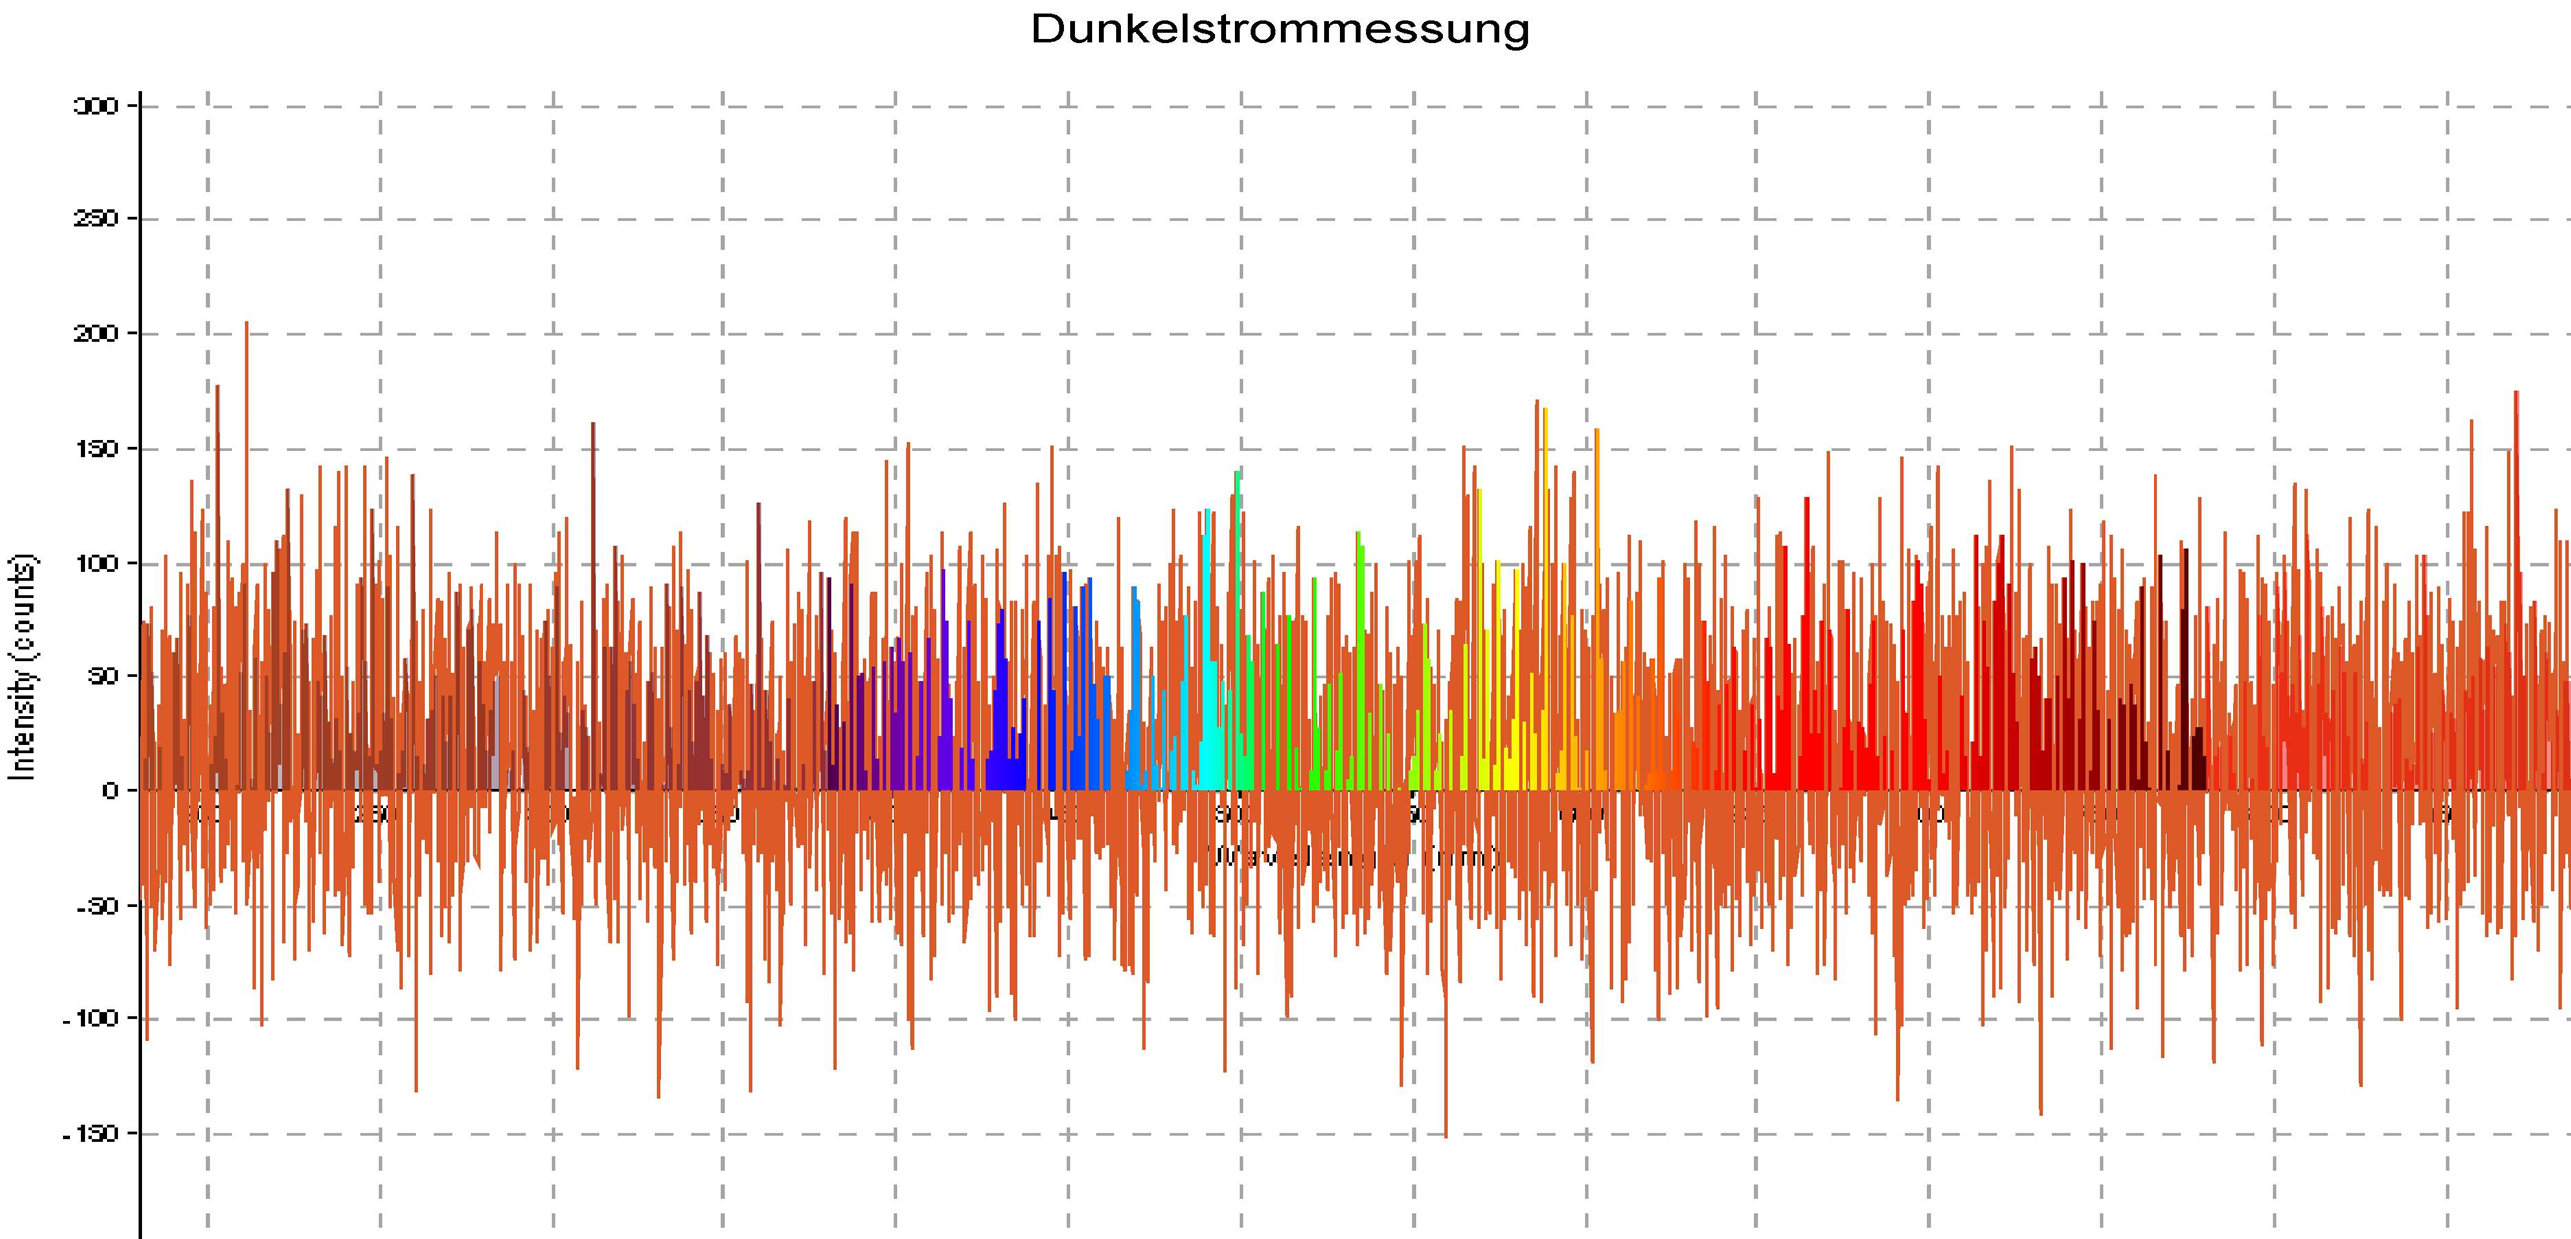
\includegraphics[width=.9\textwidth]{files/pngs/dunkelstrommessung.png}
  \caption{Spektrum Dunkelstrommessung}
  \label{fig:dunkelstrommessung}  
\end{figure}

Es handelt sich hierbei um ein Untergrundrauschen, welches wir mit der \texttt{OceanView} Software automatisch von allen weiteren aufgezeichneten Spektren abziehen.

Sofern nicht anders angegeben berechnen wir die Fehler zusammengesetzter Werte anhand der standardmäßigen Gauß'schen Fehlerfortpflanzung. Die $\sigma$-Abweichung zweier fehlerbehafteter Werte $x \pm \Delta x$ und $y \pm \Delta y$ berechnen wir anhand der Formel
\begin{align}
  \sigma = \frac{\qty|x - y|}{\sqrt{\Delta x^2 + \Delta y^2}}.
\end{align}

\subsection{Untersuchung des Sonnenlichtspektrums}

Am Tag der Versuchsdurchführung war das Wetter leider stark bewölkt, weshalb wir mit dem Spektroskop nicht auf den blauen Himmel zielen konnten. Es ist also zu beachten, dass die folgenden Betrachtungen durch die Auswirkungen der Wolkendecke gestört sind. Die untenstehende \abbref{fig:himmel_m_o_g} zeigt aufgezeichnete Spektrum des Tageslichts durch das geöffnete Fenster (blau) und durch die Fensterscheibe (orange) im Vergleich. Es ist bereits hier zu sehen, dass die Intensität durch das Glas über das gesamte Spektrum hinweg abgeschwächt wird. Die stärkste Abschwächung verzeichnen wir bei niedrigen Wellenlängen, also im UV-Bereich. Dies ist auch am Verlauf der Absorption in \abbref{fig:absorption_glas} zu sehen. Die geringste Abschwächung tritt im Bereich der Wellenlänge zwischen $400$ bis $600\si{\nano\meter}$, also dem sichtbaren Bereich auf. In Richtung des Rot- bis Infrarotbereichs steigt die Absorption wieder etwas an.

\begin{figure}[H]
  \centering
  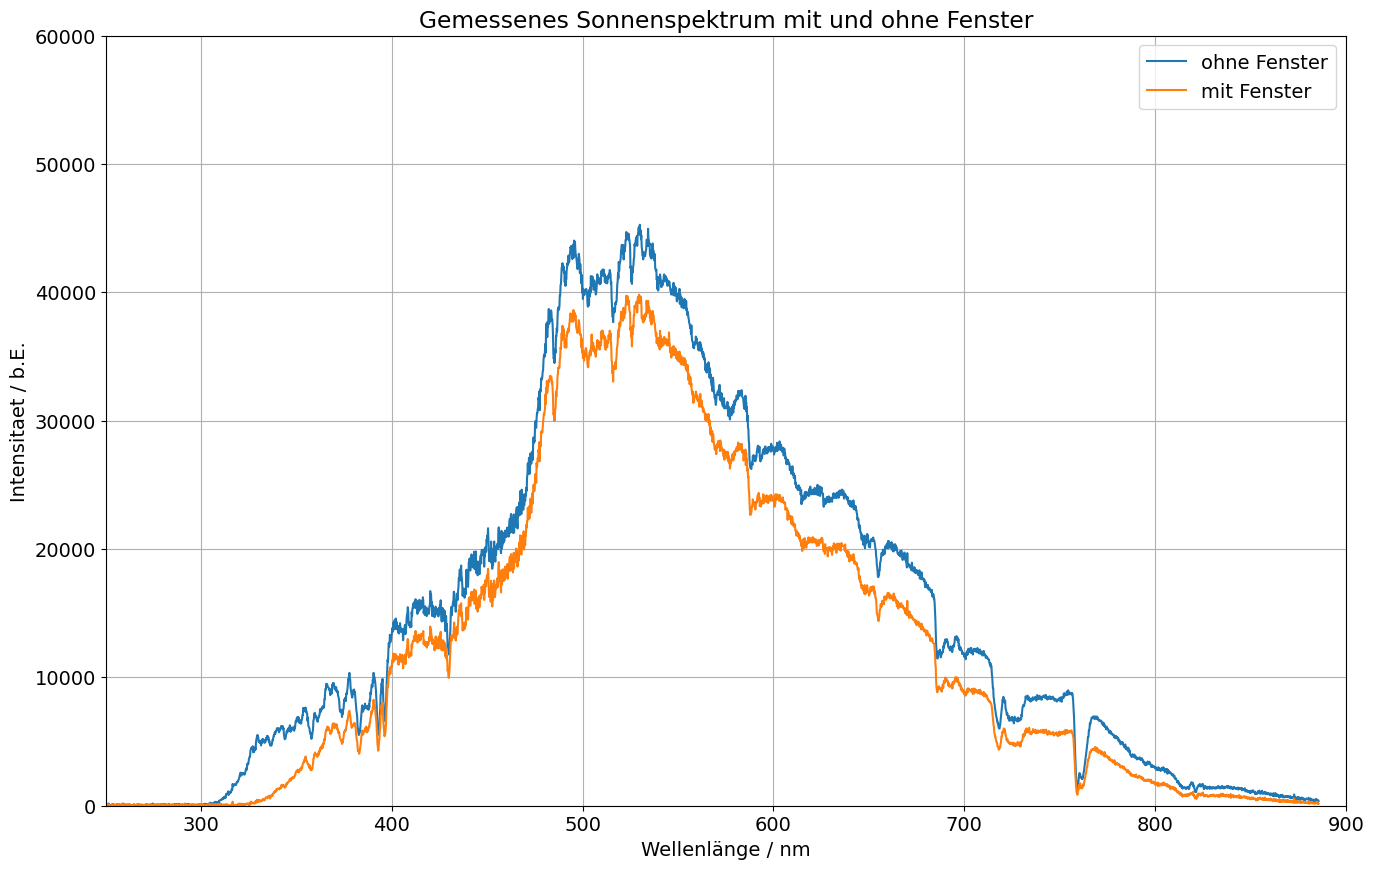
\includegraphics[width=0.8\textwidth]{files/plots/himmel_m_o_g.png}
  \caption{Sonnen}
  \label{fig:himmel_m_o_g}
\end{figure}

\begin{figure}[H]
  \centering
  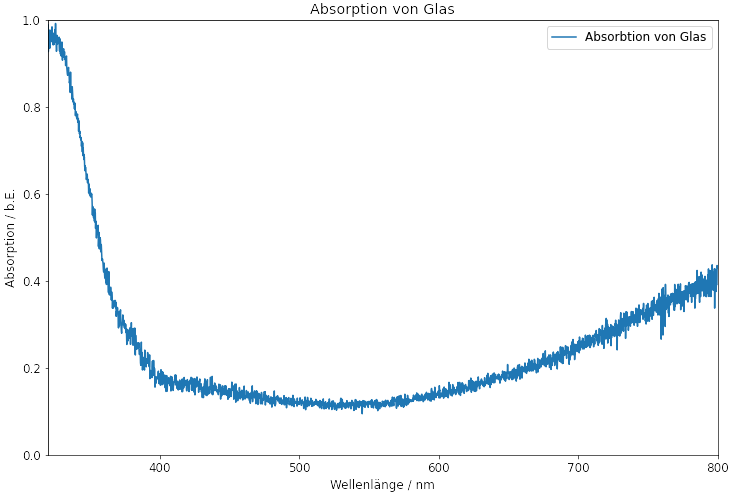
\includegraphics[width=0.8\textwidth]{files/plots/absorption_glas.png}
  \caption{Absorption}
  \label{fig:absorption_glas}
\end{figure}

Die vielen im Spektrum sichtbaren lokalen Minima sind gerade die Wellenlängen der Fraunhoferlinien, welche durch Absorption von Licht bestimmter Wellenlängen in der Sonnen- und Erdatmosphäre entstehen. \abbref{fig:spektrum_fraunhofer_balmer} zeigt erneut das Spektrum des Sonnenlichts, ohne Fensterscheibe. Markiert sind hier in Orange nun die Minima im Spektrum, welche jeweils am nächsten an der erwarteten Wellenlänge einer Fraunhoferlinie liegen. Zusätzlich sind in Grün die Literaturwerte der Wellenlänge der Balmerserie von Wasserstoff eingezeichnet.

\begin{figure}[H]
  \centering
  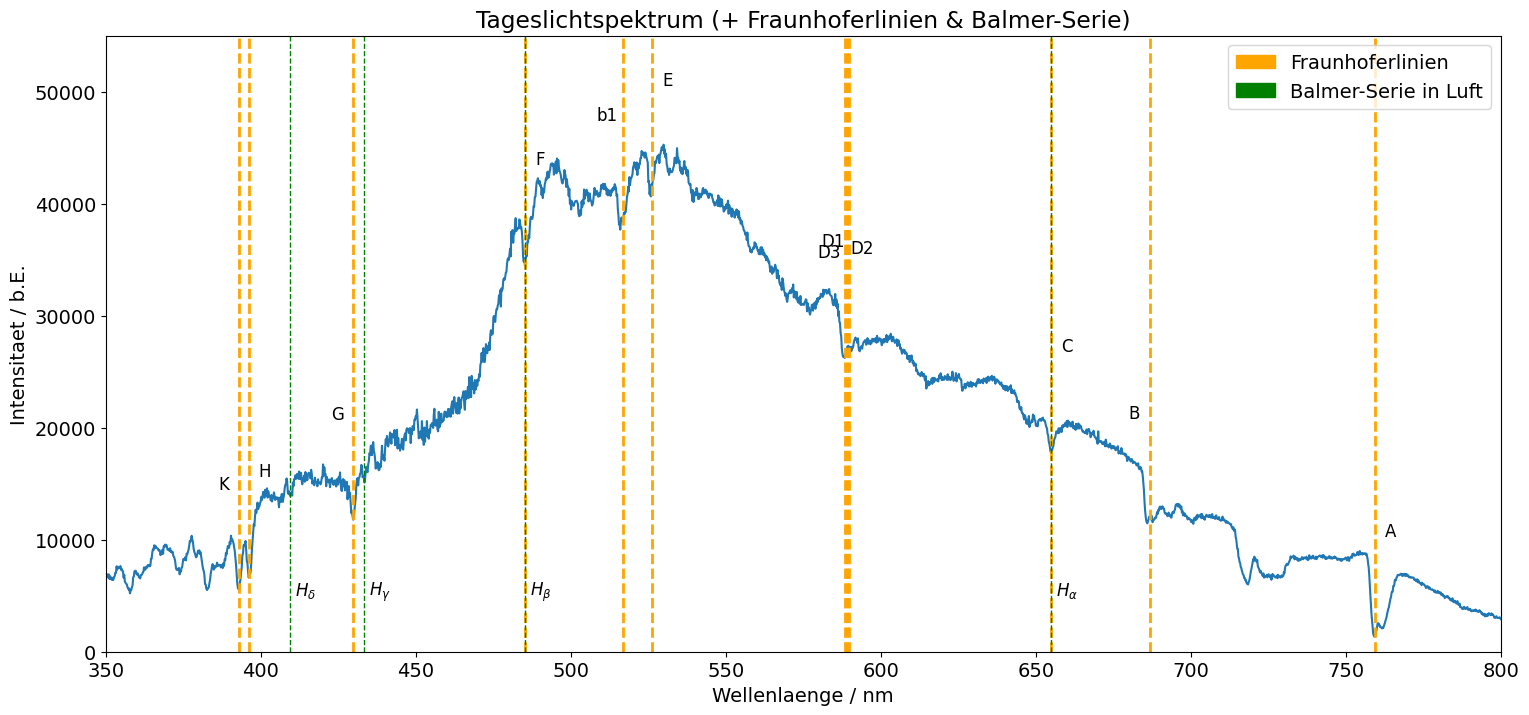
\includegraphics[width=\textwidth]{files/plots/spektrum_fraunhofer_balmer.png}
  \caption{Fraunhoferlinien und Balmerserie}
  \label{fig:spektrum_fraunhofer_balmer}
\end{figure}

\tabref{tab:fraunhofer_vergleich} zeigt eine Aufschlüsselung der erwarteten Wellenlänge der Fraunhoferlinien und der Linien der Balmerserie, die von uns aus dem Spektrum abgelesenen Werte, sowie die Abweichung zwischen den Werten. Als Fehler für die abgelesenen Wellenlängen haben wir hier einen Wert von $\pm 1 \si{\nano\meter}$ verwendet. Es ist zu sehen, dass sich die Abweichung, bis auf wenige ausnahmen auf unter einem $\sigma$ beläuft.

\begin{table}[h]
  \centering
  \caption{Vergleich der erwarteten und gemessenen Wellenlängen der Fraunhofer- und Balmerlinien}
  \vspace*{0.5em}
  \begin{tabular}{c|c|c|c}
      \hline
      Linie & Literaturwert [nm] & Abgelesener Wert [nm] & Abweichung [$\sigma$] \\
      \hline
      K  & 393.4 & 393.0 & 0.4 \\
      H  & 396.8 & 396.1 & 0.7 \\
      G  & 430.8 & 429.8 & 1.0 \\
      F  & 486.1 & 485.2 & 0.91 \\
      b1 & 518.4 & 516.7 & 1.7 \\
      E  & 527.0 & 526.2 & 0.8 \\
      D3 & 587.6 & 588.4 & 0.8 \\
      D2 & 589.0 & 589.0 & 0.0 \\
      D1 & 589.6 & 589.7 & 0.11 \\
      C  & 656.3 & 655.0 & 1.3 \\
      B  & 686.7 & 686.7 & 0.0 \\
      A  & 759.4 & 759.4 & 0.0 \\
      \hline\hline
      $\mathrm{H}_{\alpha}$ & 656.3 & 655.0 & 1.3\\
      $\mathrm{H}_{\beta}$ & 486.1 & 485.2 & 0.91\\
      $\mathrm{H}_{\gamma}$ & 434.0 & 433.4 & 0.61\\
      $\mathrm{H}_{\delta}$ & 410.1 & 409.5 & 0.61\\
      \hline
  \end{tabular}
  \label{tab:fraunhofer_vergleich}
\end{table}

\newpage

\subsection{Vergleich der Spektren verschiedener Leuchtmitte}

Im Folgenden betrachten wir die Spektren verschiedener Lichtquellen. \abbref{fig:led_vergleich} zeigt hierzu zunächst die Spektren der drei untersuchen farbigen LEDs, sowie des Lasers.

\begin{figure}[H]
  \centering
  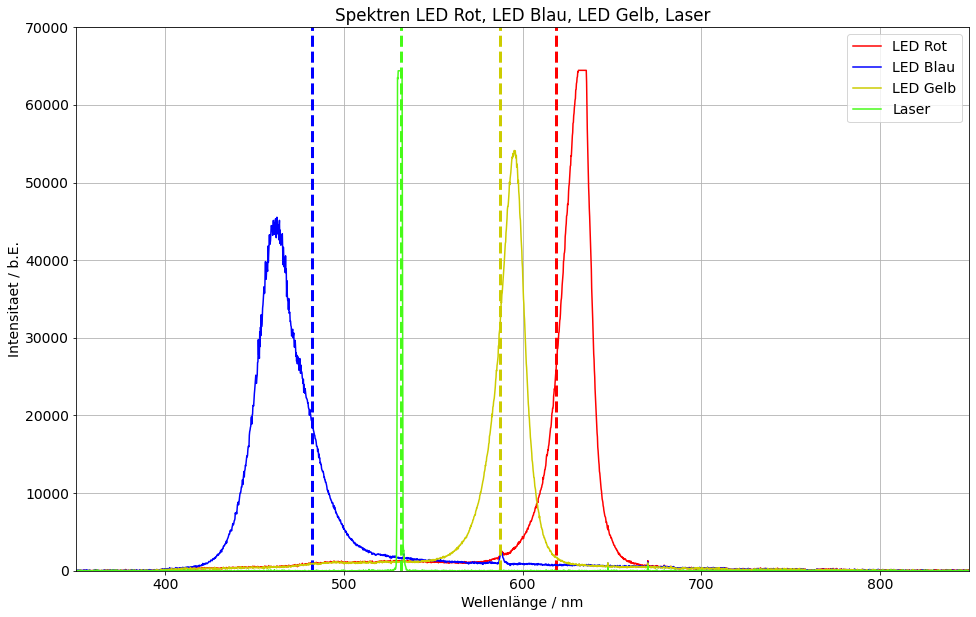
\includegraphics[width=.9\textwidth]{files/plots/led_vergleich.png}
  \caption{Aufgezeichnete Spektren der farbigen LEDs, sowie des Lasers.}
  \label{fig:led_vergleich}
\end{figure}

Die vertikalen Linien im Diagramm zeigen jeweils das nach Intensität gewichtete Mittel der Wellenlängen der Lichtquellen. Es ist zu erkennen, dass es sich hierbei in allen vier Fällen um diskrete Spektren handelt. Bei den LEDs streuen dabei die Wellenlängen etwas mehr und das Maximum der Verteilung ist etwas vom Mittel verschoben. Der Laser sendet konzentriertes Licht genau einer Wellenlänge aus, was sich ebenfalls an der direkten Überlagerung des \glqq{}Peaks\grqq{} mit dem Mittel zeigt.

Die Spektren der drei verschiedenen weißen LEDs sind gemeinsam mit dem der Energiesparlampe in \abbref{fig:led_und_energiespar} dargestellt. Alle vier Lichtquellen erzeugen, weitestgehend, weißes Licht. Am Spektrum der Energiesparlampe ist zu erkennen, dass diese das weiße Licht durch die Überlagerung mehrerer diskreter Wellenlängen erzeugt. Bei den weißen LEDs sehen wir jeweils einen relativ deutlichen, schmalen Peak bei den \glqq{}blauen\grqq{} Wellenlängen und einen sehr breiten Peak um den Bereich, in welchem Gelb zu verorten ist. Weiß wird hierbei also durch die Überlagerung von blauem und gelbem Licht erzeugt. Wir können außerdem beobachten, dass der Blau-Peak abnimmt, je \glqq{}wärmer\grqq{} das Weiß der LED wird. Durch geringere Blauanteile erhalten wir also wärmer erscheinendes Licht.

\begin{figure}[H]
  \centering
  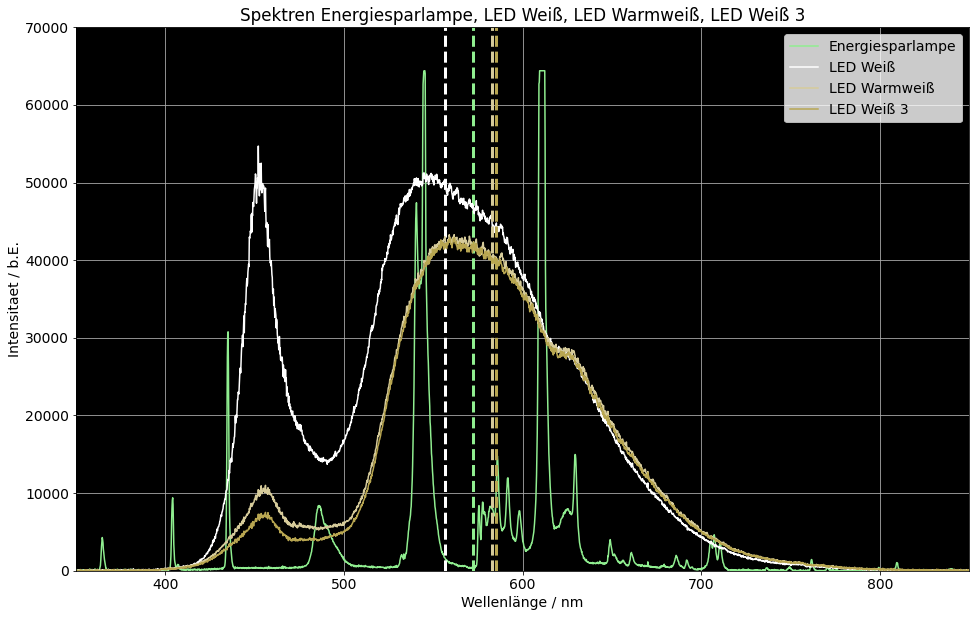
\includegraphics[width=.9\textwidth]{files/plots/led_und_energiespar.png}
  \caption{Aufgezeichnete Spektren der weißen LEDs, sowie der Energiesparlampe.}
  \label{fig:led_und_energiespar}
\end{figure}

Während die bisher betrachteten Lichtquellen Nichttemperaturstrahler sind, ist die Glühlampe ist ein Temperaturstrahler. Sie weist also ein kontinuierliches Spektrum auf, wie es auch in \abbref{fig:energiespar_und_glueh} zu sehen ist.

\begin{figure}[H]
  \centering
  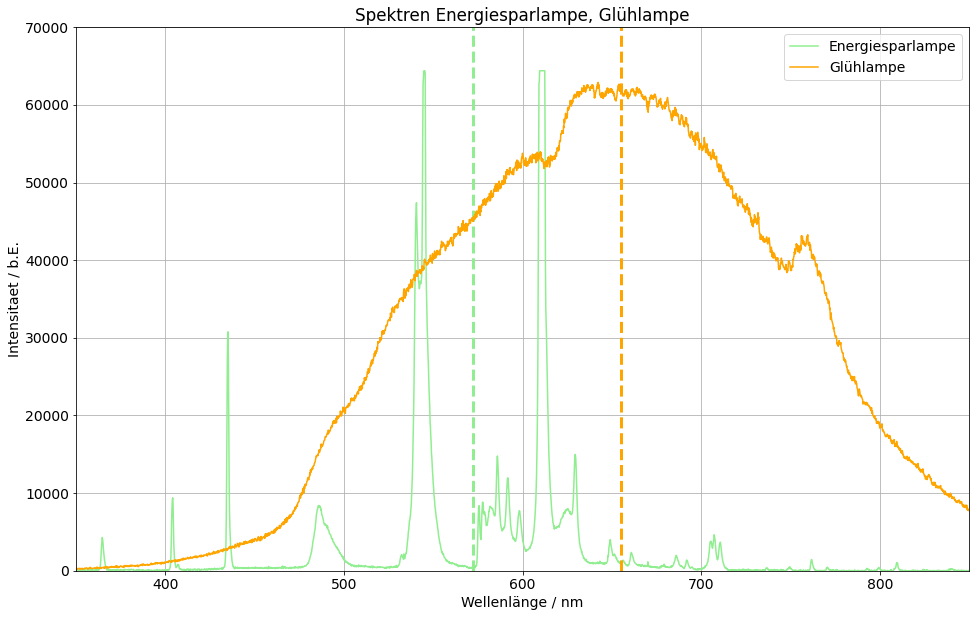
\includegraphics[width=.9\textwidth]{files/plots/energiespar_und_glueh.png}
  \caption{Aufgezeichnete Spektren der Glühlampe, sowie der Energiesparlampe.}
  \label{fig:energiespar_und_glueh}
\end{figure}

Am Spektrum der Glühlampe ist zu erkennen, dass sich ein nicht ungewisser Teil des Spektrums im oberen bis nicht sichtbaren Wellenlängenbereich befindet. Es geht hierbei also sehr viel Energie in Form von Wärme an die Umgebung verloren. Im Vergleich dazu ist die Energiesparlampe, deren Spektrum ebenfalls noch einmal in diesem Diagramm zu sehen ist, deutlich energieeffizienter. Die Glühlampe erzeugt eher ein warmes Licht, während die Lichttemperatur der Energiesparlampe eher in Richtung des kälteren Bereichs liegt.

\subsection{Untersuchung des Natriumspektrums}

\subsubsection*{Beobachtete Spektrallinien}

Im Folgenden haben wir drei verschiedene Bereiche des Spektrums einer Natriumdampflampe aufgezeichnet und möchten im weiteren Verlauf die beobachtbaren Spektrallinien mit den theoretischen Vorhersagen der Zustandsübergänge vergleichen. \abbref{fig:na_spek_350_550} zeigt die Linien geringer Intensität, welche im Bereich einer Wellenlänge von $350\si{\nano\meter}$ bis $550\si{\nano\meter}$ zu finden sind. 


\begin{figure}[H]
  \centering
  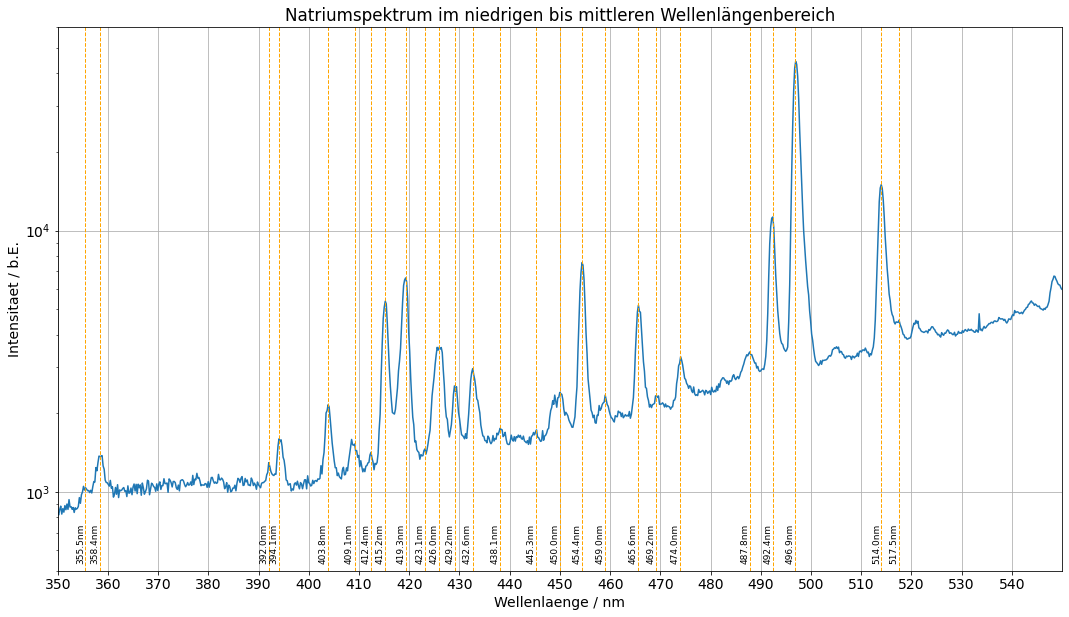
\includegraphics[width=.9\textwidth]{files/plots/na_spek_350_550.png}
  \caption{Natriuspektrum im Wellenlängenbereich von $350$ bis $550\si{\nano\meter}$.}
  \label{fig:na_spek_350_550}
\end{figure}

Als Nächstes beobachten wir den Wellenlängenbereich zwischen $585$ und $595\si{\nano\meter}$. In diesem ist die markante D-Linie des Natriumspektrums zu finden. Die Intensität der D-Linie ist im Vergleich zu den anderen Linien so hoch, dass keine weiteren Linien im aufgezeichneten Spektrum sichtbar sind, wenn die D-Linie nicht in Sättigung ist. Diesen Fall zeigt die \abbref{fig:na_spek_dlinie_nichtsaett}. Ebenfalls relativ gut zu erkennen ist in dieser Abbildung die Doppelstruktur der D-Linie aus zwei dicht beieinander liegenden Linien.


\begin{figure}[H]
  \centering
  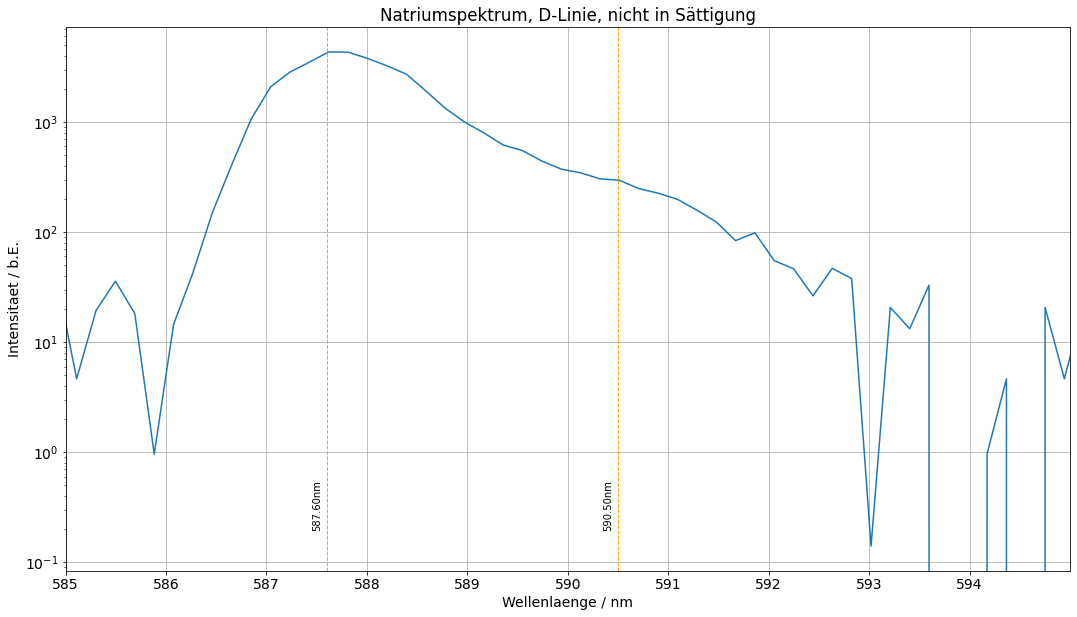
\includegraphics[width=.9\textwidth]{files/plots/na_spek_dlinie_nichtsaett.png}
  \caption{D-Linie im Natriumspektrum, nicht in Sättigung.}
  \label{fig:na_spek_dlinie_nichtsaett}
\end{figure}

Betrachten wir einen etwas weiteren Wellenlängenbereich um die D-Linie, erlauben dieser allerdings in Sättigung zu gehen, so können wir in deren Umgebung weitere Spektrallinien geringer Intensität beobachtbaren. Diese sind in \abbref{fig:na_spek_dlinie_saett} gekennzeichnet.

\begin{figure}[H]
  \centering
  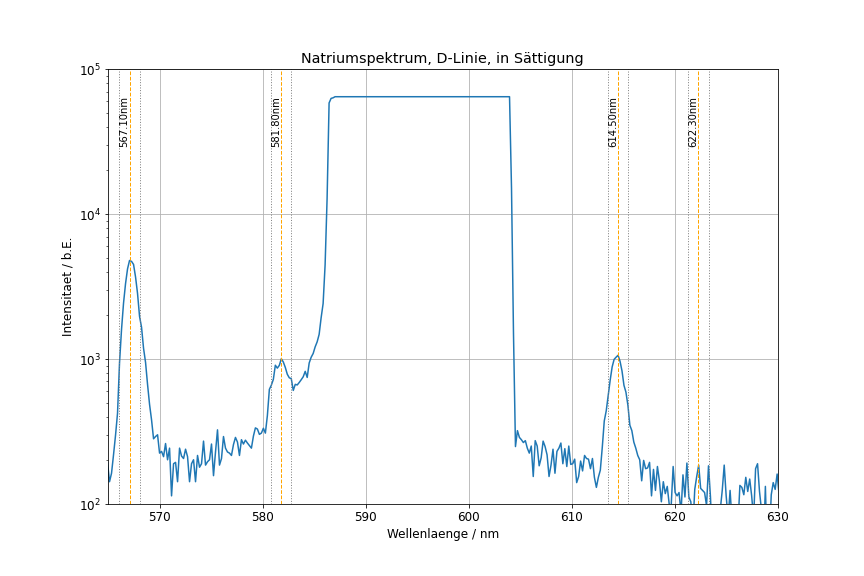
\includegraphics[width=.9\textwidth]{files/plots/na_spek_dlinie_saett.png}
  \caption{Weitere Linien um die D-Linie im Natriumspektrum, während diese in Sättigung ist.}
  \label{fig:na_spek_dlinie_saett}
\end{figure}

Als letztes Betrachten wir den oberen Bereich des Natriumspektrums von $650$ bis $850\si{\nano\meter}$. Wie in \abbref{fig:na_spek_650_850} zu sehen sind hier wieder sehr viele, teils auch sehr markante, Spektrallinien aufzufinden. 


\begin{figure}[H]
  \centering
  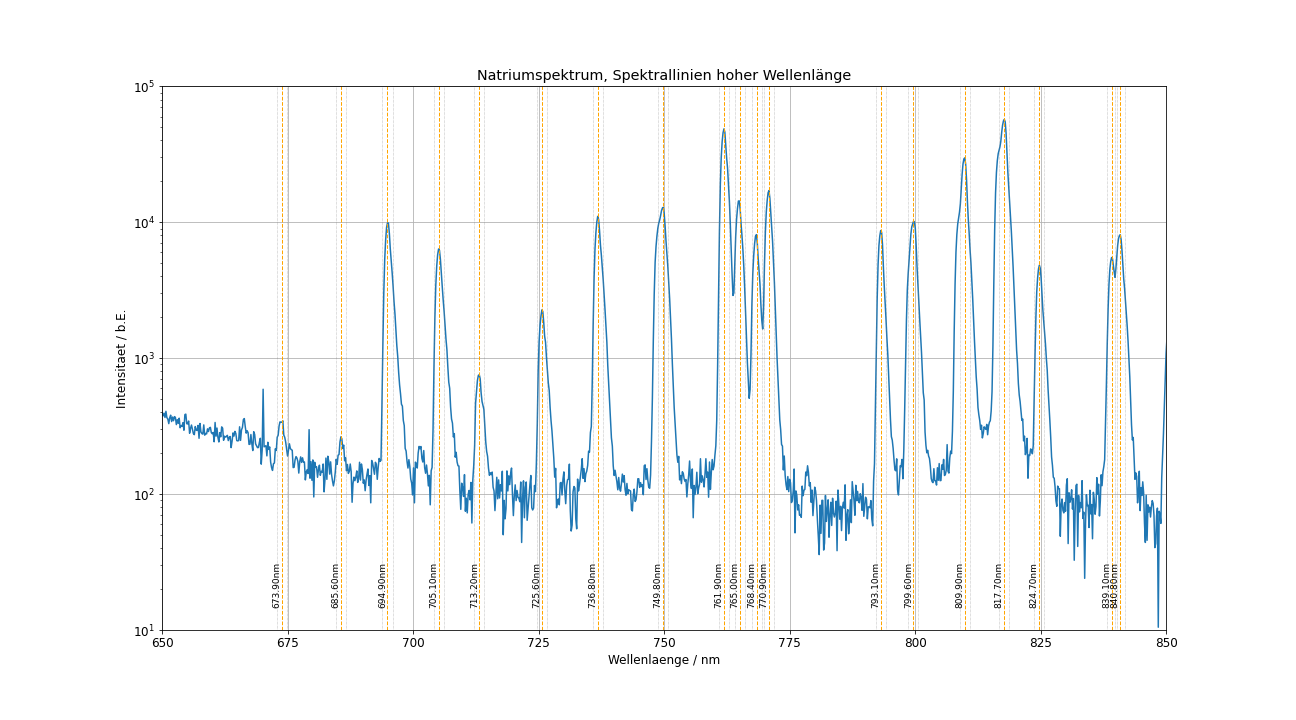
\includegraphics[width=.9\textwidth]{files/plots/na_spek_650_850.png}
  \caption{Natriumspektrum im Wellenlängenbereich von $350$ bis $550\si{\nano\meter}$.}
  \label{fig:na_spek_650_850}
\end{figure}

Nun möchten wir die beobachteten Spektrallinien mit den Vorhersagen der Theorie vergleichen.

\subsubsection*{Erwartete Linien für die 1. Nebenserie $md \to 3p$}

\textit{Vorbemerkung: In den folgenden Berechnungen gehen wir für die Konstanten von den Werten $E_{Ry} = -13.605\si{\electronvolt}$ und $hc = 1.2398 * 10^3 \si{\nano\meter \electronvolt}$ aus.}

Den Korrekturterm $\Delta_{d}$ können wir für diese Serie vernachlässigen. Für die Wellenlänge $\lambda_m$ für die Übergänge $md \to 3p$ gilt
\begin{align}
  \lambda_m &\approx \frac{hc}{\frac{E_{Ry}}{m^2} - E_{3p}}.
\end{align}
Hierbei sind die Rydbergenergie $E_{Ry} = -13.605\unit{\electronvolt}$, sowie $hc = 1.2398 \cdot 10^{3} \si{\nano\meter \electronvolt}$ als Konstanten gesetzt. $E_{3p}$ können wir mit dieser Formel berechnen, indem wir $m = 3$ und entsprechend $\lambda_3$ gleich der gemessenen Linie im Bereich von $819\si{\nano\meter}$ setzen. Die von uns gemessene Linie, welche am nächsten an dieser ist, liegt bei $817.7\si{\nano\meter}$. Damit erhalten wir einen Wert von
\begin{align}
  E_{3p} = -3.0279 \pm 0.0019\si{\electronvolt}.
\end{align}

Setzen wir nun diese Energie und die Quantenzahl $m$ im Bereich von $3$ bis $12$ in die obige Formel ein, so erhalten wir die erwarteten Wellenlängen für die jeweiligen Übergänge. Diese sind in \tabref{tab:wellenlaengen_1ns} zu sehen, gemeinsam mit der zugeordneten Spektrallinie aus unseren Beobachtungen, sowie der jeweiligen Abweichung.

\begin{table}[H]
  \centering
  \caption{Vergleich der berechneten und gemessenen Wellenlängen der 1. Nebenserie $md \to 3p$.}
  \vspace*{0.5em}
  \begin{tabular}{c c c c}
      \hline
      $m$ & $\lambda_{\text{theo.}}$ [nm] & $\lambda_{\text{beob.}}$ [nm] & Abweichung \\
      \hline
      3  & $817.7 \pm 1.000$ & $817.7 \pm 1$ & 0.01$\sigma$ \\
      4  & $569.4 \pm 0.5$ & $567.1 \pm 1$ & 2.03$\sigma$ \\
      5  & $499.2 \pm 0.4$ & $496.9 \pm 2$ & 1.13$\sigma$ \\
      6  & $467.9 \pm 0.4$ & $469.2 \pm 1$ & 1.28$\sigma$ \\
      7  & $450.8 \pm 0.4$ & $450.0 \pm 1$ & 0.77$\sigma$ \\
      8  & $440.4 \pm 0.3$ & $438.1 \pm 1$ & 2.20$\sigma$ \\
      9  & $433.5 \pm 0.3$ & $432.6 \pm 1$ & 0.88$\sigma$ \\
      10 & $428.7 \pm 0.3$ & $429.2 \pm 1$ & 0.46$\sigma$ \\
      11 & $425.3 \pm 0.3$ & $426.0 \pm 1$ & 0.72$\sigma$ \\
      12 & $422.7 \pm 0.3$ & $423.1 \pm 1$ & 0.44$\sigma$ \\
      \hline
  \end{tabular}
  \label{tab:wellenlaengen_1ns}
\end{table}

\subsubsection*{Erwartete Linien für die 2. Nebenserie $ms \to 3p$}

Bei der Betrachtung der 2. Nebenserie können wir den Korrekturterm $\Delta_s$ nicht vernachlässigen. Die Bindungsenergie des Grundzustandes $E_{3s}$ berechnen wir nach der Formel
\begin{align}
  E_{3s} = E_{3p} - \frac{hc}{\lambda}.
\end{align}

Für die Wellenlänge $\lambda$ setzen wir die beobachtete Wellenlänge der D-Linie ein, da diese dem Übergang $3p \to 3s$ entspricht. In unseren Aufzeichnungen können wir diese Linie bei in etwa $\lambda = (590.5 \pm 1) \si{\nano\meter}$ beobachten. Damit erhalten wir eine Bindungsenergie von
\begin{align}
  E_{3s} = (-5.127 \pm 0.005) \si{\electronvolt}.
\end{align}
Durch Umstellen der Gleichung
\begin{align}
  E_{3s} = \frac{E_{Ry}}{(3 - \Delta_s)^2}
\end{align}
berechnen wir den Wert des Korrekturterms zu
\begin{align}
  \Delta_s = 1.3711 \pm 0.0007.
\end{align}

Die erwarteten Werte für die Wellenlängen der Linien können wir dann pro Quantenzahl $m$ mit der Formel
\begin{align}
  \lambda_m \approx \frac{hc}{\frac{E_{Ry}}{(m - \Delta_s)^2} - E_{3p}}
\end{align}
berechnen. Die Werte für $m$ im Bereich von $4$ bis $9$ sind in der \tabref{tab:wellenlaengen_2ns} wiederzufinden. Zur Berechnung der Fehler der $\lambda_m$ haben wir hierbei, aufgrund der Komplexität der Formel, auf eine relative Fehlerbetrachtung zurückgegriffen.

\begin{table}[H]
  \centering
  \caption{Vergleich der berechneten und gemessenen Wellenlängen der 2. Nebenserie $ms \to 3p$.}
  \vspace*{0.5em}
  \begin{tabular}{c c c c}
      \hline
      $m$ & $\lambda_{\text{theo.}}$ [nm] & $\lambda_{\text{beob.}}$ [nm] & Abweichung \\
      \hline
      4  & $1170.4 \pm 1.4$ & -     & -     \\
      5  & $621.5 \pm 0.7$  & $622.3 \pm 1$ & $0.67\sigma$ \\
      6  & $518.1 \pm 0.6$  & $517.5 \pm 1$ & $0.53\sigma$ \\
      7  & $477.1 \pm 0.6$  & $474.0 \pm 1$ & $2.76\sigma$ \\
      8  & $456.1 \pm 0.6$  & $454.4 \pm 1$ & $1.52\sigma$ \\
      9  & $443.7 \pm 0.5$  & $445.3 \pm 1$ & $1.42\sigma$ \\
      \hline
  \end{tabular}
  \label{tab:wellenlaengen_2ns}
\end{table}

\subsubsection*{Erwartete Linien für die Hauptserie $mp \to 3s$}

Zu guter Letzt betrachten wir noch die erwarteten Linien der Hauptserie $mp \to 3s$. Hierzu benötigen wir den Korrekturterm $\Delta_p$, welchen wir ähnlich zur vorherigen Betrachtung durch Umstellen der Gleichung
\begin{align}
  E_{3p} = \frac{E_{Ry}}{(3 - \Delta_p)^2}
\end{align}
zu
\begin{align}
  \Delta_p = 0.8803 \pm 0.0007
\end{align}
berechnen.

Mit diesem Wert berechnen wir nach der Gleichung
\begin{align}
  \lambda_m \approx \frac{hc}{\frac{E_{Ry}}{(m - \Delta_p)^2} - E_{3s}}
\end{align}
die erwarteten Wellenlängen der Linien mit den Quantenzahlen $m = 4$ und $5$. Diese sind in der \tabref{tab:wellenlaengen_hs} zu finden. Da wir den Bereich des Spektrums, in dem sich diese Linien befinden, nicht aufgezeichnet haben, können wir diese nicht mit beobachteten Werten vergleichen.

\begin{table}[H]
  \centering
  \caption{Berechneten Wellenlängen der Hauptserie $mp \to 3s$.}
  \vspace*{0.5em}
  \begin{tabular}{c c c c}
      \hline
      $m$ & $\lambda_{\text{theo.}}$ [nm] & $\lambda_{\text{beob.}}$ [nm] & Abweichung \\
      \hline
      4  & $332.4 \pm 0.6$ & -     & -     \\
      5  & $286.6 \pm 0.5$  & - & - \\
      \hline
  \end{tabular}
  \label{tab:wellenlaengen_hs}
\end{table}

\subsection{Bestimmung der Serienenergien und der l-abhängigen Korrekturfaktoren}

Die Funktionen, welche wir bisher genutzt hatten, um die Wellenlängen der Spektrallinie berechnen, können wir umgekehrt auch verwenden um die Rydbergenergie, sowie die Korrekturterme zu berechnen. Dazu tragen wir die gemessenen Wellenlängen der ersten Nebenserie in ein Diagramm auf und Fitten an diese Daten die Funktion
\begin{align}
  \lambda_m = \frac{hc}{\frac{E_{Ry}}{(m-\Delta_d)^2} - E_{3p}}.
\end{align}

Hierbei lassen wir $E_{Ry}, E_{3p}$ und $\Delta_d$ freie Parameter, welche wir mit den Startwerten 
\begin{align}
  E_{Ry} = -13.6\, [\si{\electronvolt}], \quad
  E_{3p} = -3\, [\si{\electronvolt}], \quad
  \Delta_d = -0.02
\end{align}
vorbelegen. \abbref{fig:na_1ns_fit} zeigt die aufgetragenen Messdaten sowie das grafische Resultat des Fits.

\begin{figure}[H]
  \centering
  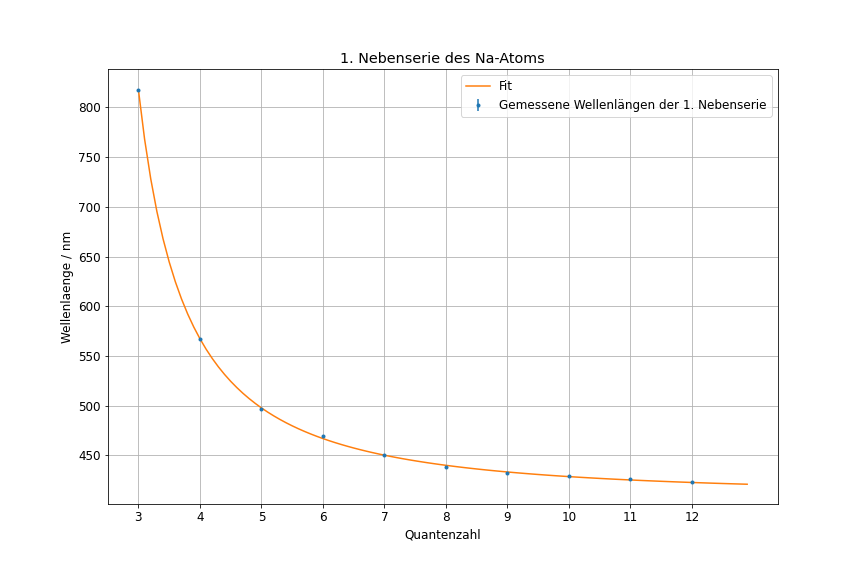
\includegraphics[width=.9\textwidth]{files/plots/na_1ns_fit.png}
  \caption{Resultat für den Fit an die Wellenlängen der 1. Nebenserie.}
  \label{fig:na_1ns_fit}
\end{figure}

Die durch den Fit optimierten Werte der Parameter entsprechen
\begin{align}
  E_{Ry} = -13.0 \pm 0.5\, [\si{\electronvolt}], \quad
  E_{3p} = -3.023 \pm 0.006\, [\si{\electronvolt}], \quad
  \Delta_d = 0.07 \pm 0.05.
\end{align}

Die Güte des Fits bestimmen wir durch das Berechnen der $\chisq$-Summe nach
\begin{align}
  \chisq = \sum_{i}^{N} \qty(\frac{\text{Funktionswert}_i - \text{Messwert}_i}{\text{Fehler}_i})^2,
\end{align}
sowie dem reduzierten $\chisq$-Wert nach $\chisqrd = \flatfrac{\chisq}{\#\text{Freiheitsgrade}}$.

Aus dem gezeigten Fit erhalten wir für diese Werte von
\begin{align}
  \chisq = 10.53,\qquad \chisqrd = 1.50.
\end{align}

Für die Fitwahrscheinlichkeit erhalten wir einen Wert von $16.0\%$.

Den gleichen Prozess führen wir nun noch einmal für die 2. Nebenserie durch. Dafür fitten wir die Funktion
\begin{align}
  \lambda_m = \frac{hc}{\frac{E_{Ry}}{(m - \Delta_s)^2} - E_{3p}}
\end{align}
an die gemessenen Wellenlängen. Die Variablen initialisieren wir erneut mit den Startwerten
\begin{align}
  E_{Ry} = -13.6\, [\si{\electronvolt}], \quad
  E_{3p} = -3\, [\si{\electronvolt}], \quad
  \Delta_s = 1.5.
\end{align}

Das grafische Resultat ist in \abbref{fig:na_2ns_fit} zu sehen.

\begin{figure}[H]
  \centering
  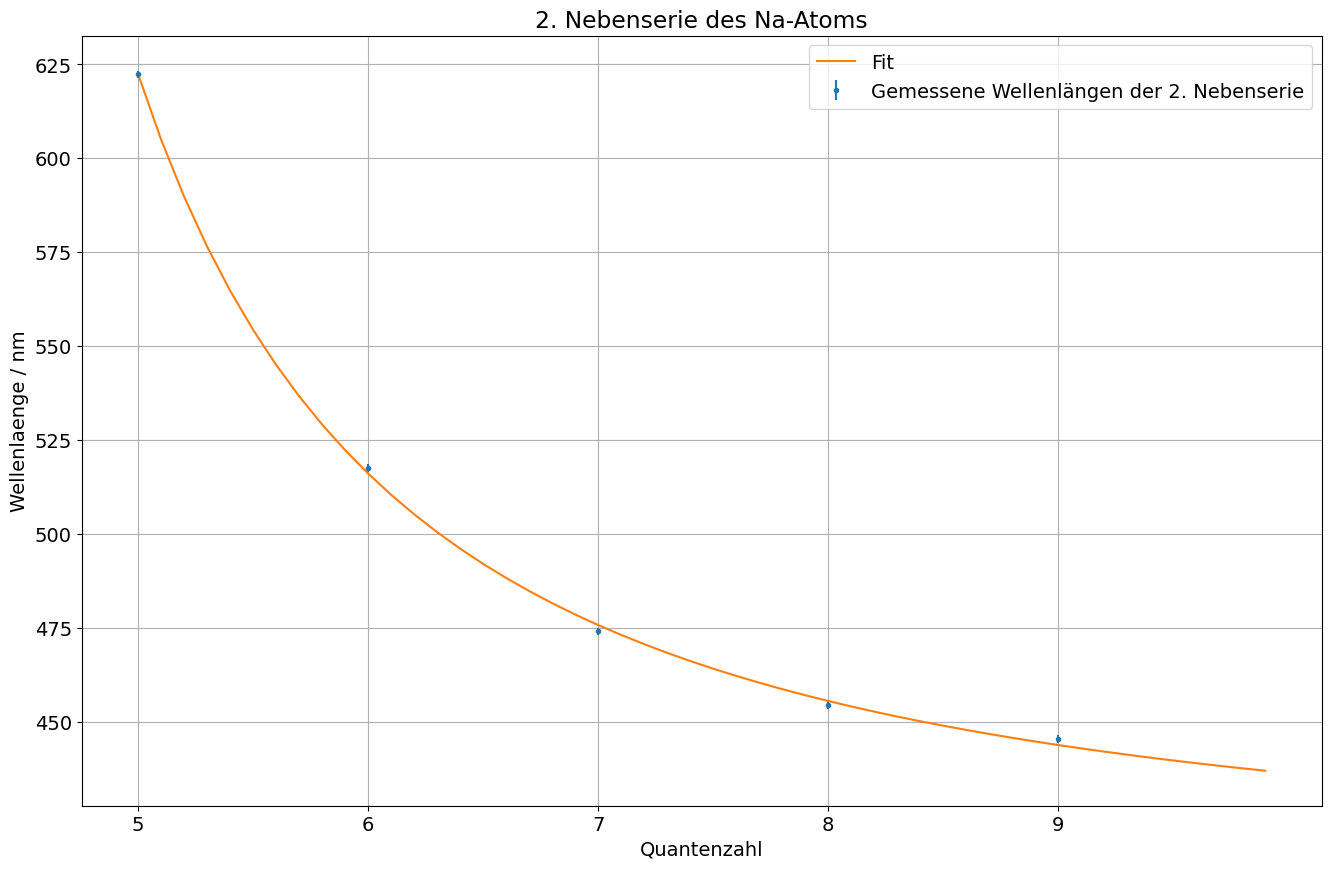
\includegraphics[width=.9\textwidth]{files/plots/na_2ns_fit.png}
  \caption{Resultat für den Fit an die Wellenlängen der 2. Nebenserie.}
  \label{fig:na_2ns_fit}
\end{figure}

Wir erhalten die folgenden optimierten Werte für die Variablen:
\begin{align}
  E_{Ry} = -11.6 \pm 2.1\, [\si{\electronvolt}], \quad
  E_{3p} = -3.01 \pm 0.04\, [\si{\electronvolt}], \quad
  \Delta_s = 1.62 \pm 0.25.
\end{align}

Die Güte des Fits wird mit
\begin{align}
  \chisq = 8.55,\qquad \chisqrd = 4.28.
\end{align}
bewertet und die Fitwahrscheinlichkeit beläuft sich auf einen Wert von $1.0\%$.